\section{Experiments and Results}
In this section we present results from experiments over our data sets. Since our work involves the novel definitions of Elemental and Composite concepts in learning modules' Concept Profiles, we do not have any baselines to compare our method against. Thus we will provide thorough qualitative analysis from each of our data sets, as well as error analysis for these qualitative results. The quantitative analysis will depend instead on expert feedback from one instructor on two of our data sets. We also provide our open source results and instructor gold standards for these two data sets as a freely available baseline for any future work in this area.

\subsection{Data Sets}
Our data consists of two textbooks and four MOOC courses's lecture transcripts. The textbooks are: 1) "Text Data Management and Analysis: A Practical Introduction to Information Retrieval and Text Mining" by ChengXiang Zhai and Sean Massung \cite{} , 2) Third edition of "Data Mining: Concepts and Techniques" by Jaiwei Han, Micheline Kamber, and Jian Pei \cite{}. Both textbooks are available open source through the first authors' web pages. The four MOOC courses courses 2 to 5 in the Data Mining Specialization on Coursera.\footnote{\url{https://www.coursera.org/specializations/data-mining}.} Namely: 1) Text Retrieval and Search Engines, 2) Text Mining and Analytics, 3) Pattern Discovery in Data Mining, and 4) Cluster Analysis in Data Mining. All four MOOCs' lecture transcripts can be freely obtained from Coursera.

We chose this particular collection of data sets for several reasons: first, the first two MOOCs cover roughly the same material as the first textbook, while the last two MOOCs cover roughly the same material as the second textbook. Thus, we are able to train our biLSTM on each of the textbooks and their indices and then run it on the corresponding MOOC data to extract high quality concept phrases. The second reason is that the first authors of the textbooks are the instructors who designed each of the corresponding MOOC courses. This increases the quality of the concept extraction results as well since ambiguity and variation of concept phrases are at a minimum. Table \ref{} shows some statistics about our textbook data sets, and table \ref{} shows some statistics about our MOOC data sets.

%ADD TABLES FOR TEXTBOOK AND MOOC DATA: NUMBER OF WORDS, LENGTH OF INDEX FOR TEXTBOOK, NUMBER OF LECTURES FOR MOOC.

\subsection{Experiment Design}
For our experiment, we trained two LSTM models one on each textbook. We ran the first trained LSTM model on MOOC1 and MOOC2, and the second trained LSTM model on MOOC3 and MOOC4 to extract concept phrases from the respective MOOC's lecture transcripts. Table \ref{} shows statistics for the extracted concepts from the four MOOCs.
For each one of our six data sets (2 textbooks and 4 MOOCs), we ran the Layered Fuzzy C-Means clustering algorithm to get the clusters and retained layers and the ranked list of concepts and their EC Scores. Detailed parameter values and experimental results are presented in \ref{exp_results}. 

\subsection{Experiment Results}\label{exp_results}
% AIDAN: are there any initialization parameters for the concept extraction LSTM?
Table \ref{} presents the initialization values for the parameters $INIT\_CLUSTERS$, $min_p$, and $min_q$ for each of our data sets when running the Layered Fuzzy C-Means algorithm. The following subsection \ref{qualitative} discusses the qualitative results obtained from these runs and presents visualizations for the layer clusters and EC Scores. For the purpose of visualizations, all data points have been reduced from 64 dimensional vectors to 2D vectors using Principal Component Analysis.

\subsubsection{Qualitative Analysis}\label{qualitative}

%Here we show sample ranked lists (top-k) for multiple MOOCs, and discuss the quality of the results. We want to show that they can indeed be useful to help learners assess the pre-requisite and the major concepts taught in a module. 
Figure \ref{han_clusters} shows the retained layers and clusters for Textbook 1: "Data Mining: Concepts and Techniques". The left top-most subplot of the figure shows all data points in the input matrix $X$ plotted in 2D. Each subsequent subplot represents a retained layer from the Layered Fuzzy C-Means algorithm and the "hard border" clusters in that layer. As you can see, we retain 21 layers for Textbook 1. Figure \ref{han_layer_qual} shows the retained layers (labeled in blue) against their Calinski Harabaz Index for clustering quality. All plotted layers have passed the CH Index threshold, but we further drop the layers (labeled in grey) that have less than two data point plotted as belonging to clusters in that layer, or for which $\sum H_{i} \leq 1$. Figure \ref{han_EC} plots the extracted concepts versus their EC Score sorted in a decreasing order. We can see from the figure that "randomization methods" is more Elemental than "attribute construction" which is more Elemental than "fuzzy clustering". Figures \ref{} to \ref{} present the visual results for Textbook 2: "Text Data Management and Analysis: A Practical Introduction to Information Retrieval and Text Mining", and Figures \ref{} to \ref{} present the visual results for MOOC 1 through 4. 

\begin{figure*}[t]
	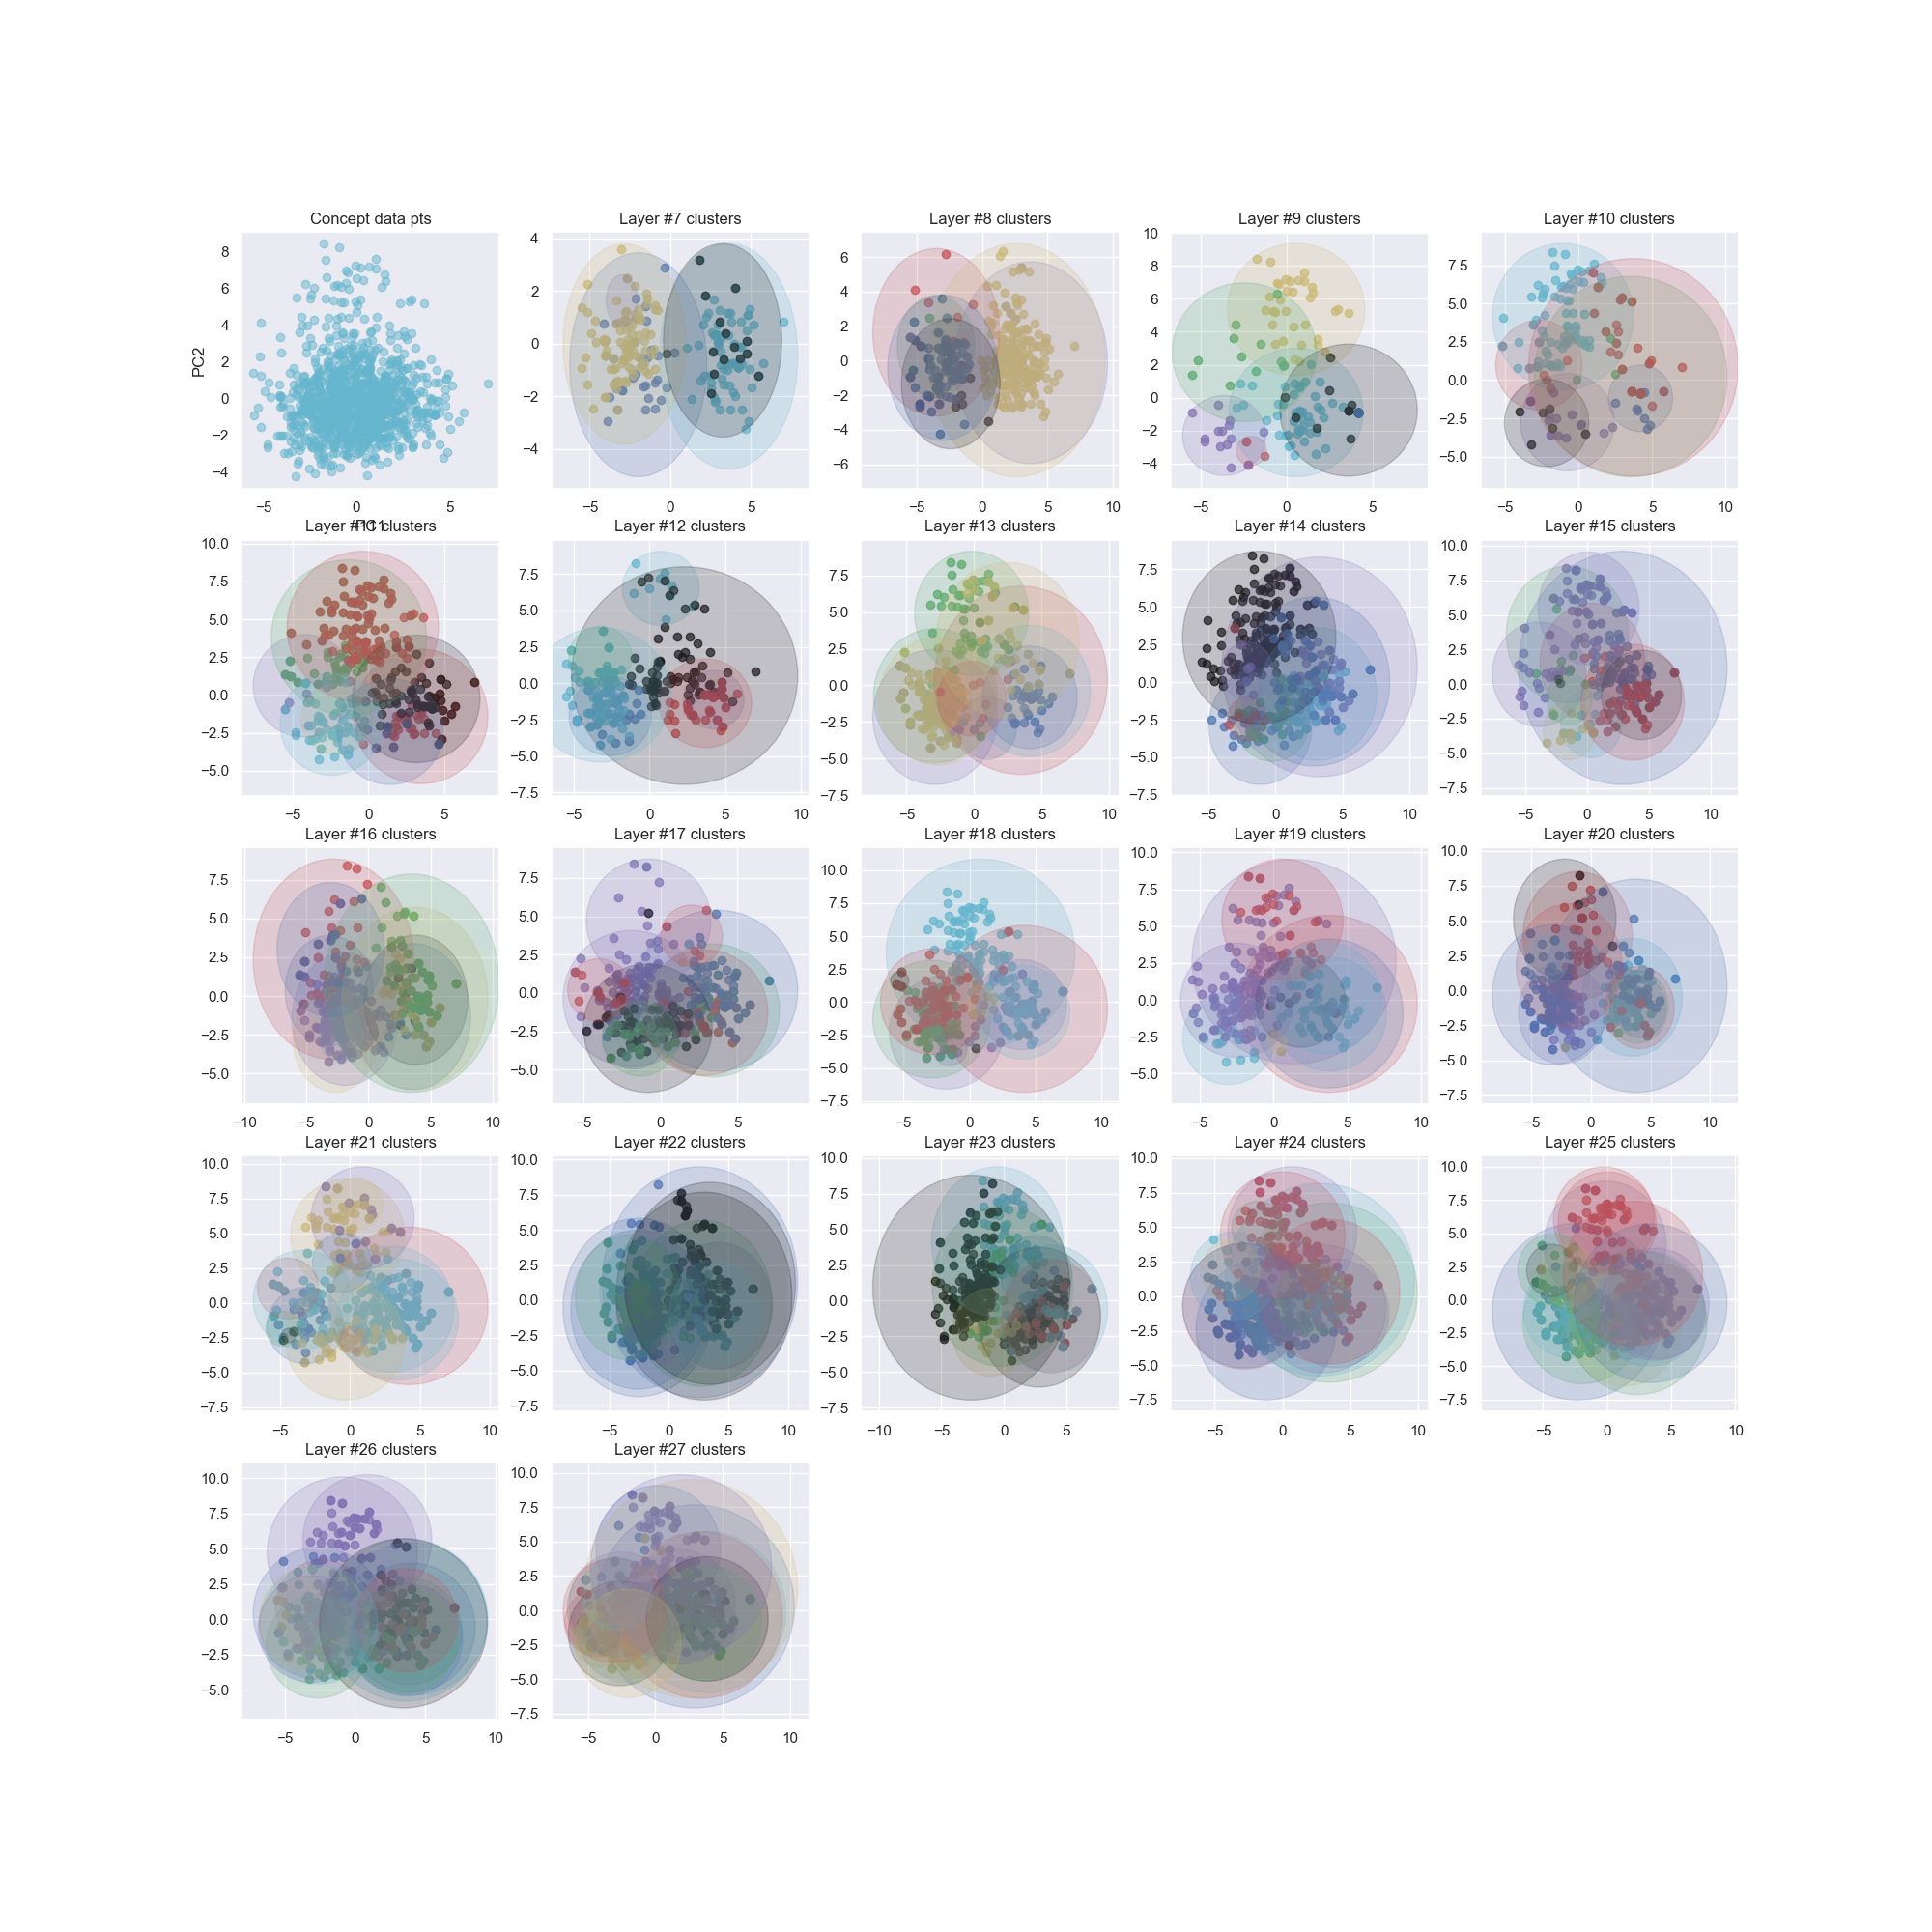
\includegraphics[width=0.5\textwidth, left]{figures/han_bidi_clusters_1.png}
	\caption{Retained layers and clusters for Textbook 1: "Data Mining: Concepts and Techniques"}
	\label{han_clusters}
\end{figure*}

\begin{figure*}[t]
	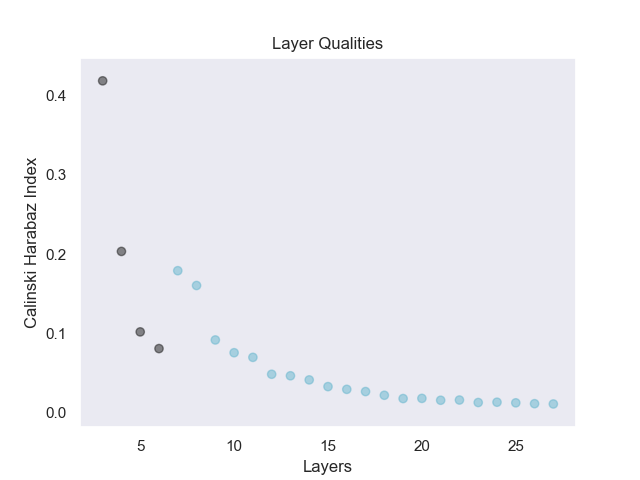
\includegraphics[width=0.5\textwidth, left]{figures/han_bidi_layer_qual_1.png}
	\caption{CH Index for layer quality for Textbook 1: "Data Mining: Concepts and Techniques"}
	\label{han_layer_qual}
\end{figure*}

\begin{figure*}[t]
	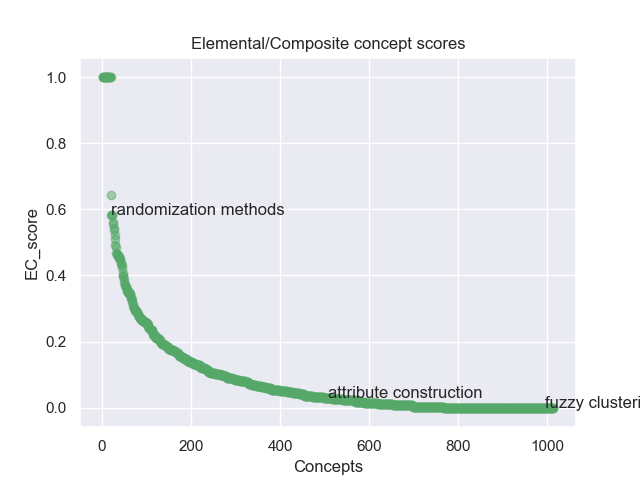
\includegraphics[width=0.5\textwidth, left]{figures/han_bidi_EC_scores_good1.png}
	\caption{Decreasing EC Score for Textbook 1 concepts}
	\label{han_EC}
\end{figure*}

\subsubsection{Quantitative Analysis}\label{quantitative}
% AIDAN: ADD RESULTS FOR THE LSTM AND THE PLOTS OF THE ACCURACY/F1 SCORE 

%Here we use the Text Retrieval MOOC to do quantitative evaluation, mainly to compare different methods and see which method is the best or examine how we can improve the accuracy. But we can also quantify the accuracy to understand the utility of the proposed methods. 
%This should allow us to draw conclusions about which method/idea works the best.

\subsubsection{Error analysis}\label{error}

%Do some analysis to understand where the proposed methods make mistakes. This helps identifying additional challenges for future study. 
